\chapter{Methods in Trainig and Testing The Model}

\section{Methodology}
For this project as in most image classification it can be split up into:
\begin{itemize}
    \item Data Preparation
    \item Model Training
    \item Model Testing and Evaluation
\end{itemize}

\subsection{Data Preparation}
The dataset for this project, consisting of images of various animal species, was  from Kaggle. Unfortunately, this dataset did not come pre-split into training and testing subsets. This meant i had to do i myself. I could have just used it as is, and for testing data use some from google, but i decided this was faster than going around installing images one by one from google images.


The dataset was structured with separate folders for each category of animals, each category folder containing respective images. So i created a python script that redistributed these images into two new folders: one for training and another for testing. 90\% of the images were allocated to the training set, and the remaining 10\% were reserved for the test set. I decided not to do the normal rule of thumb when splitting data 70:30 because images of all these animals are easily accessible from google. Also the dataset was only 38 megabyte, so i decided the model having more images to train om would increase the accuracy.

Fortunately sklearn has a function that does this already so i used that. 

\begin{lstlisting}[language=Python]
    import os
    import shutil
    from sklearn.model_selection import train_test_split
    
    current_script_path = os.path.dirname(os.path.abspath(__file__))
    
    data_dir = os.path.join(current_script_path, 'animal_data')
    print(data_dir)
    
    categories = os.listdir(data_dir)
    
    train_dir = os.path.join(current_script_path, 'training')
    test_dir = os.path.join(current_script_path, 'testing')
    
    os.makedirs(train_dir, exist_ok=True)
    os.makedirs(test_dir, exist_ok=True)
    
    for category in categories:
        category_path = os.path.join(data_dir, category)
        images = os.listdir(category_path)
        
        train_cat_dir = os.path.join(train_dir, category)
        test_cat_dir = os.path.join(test_dir, category)
        os.makedirs(train_cat_dir, exist_ok=True)
        os.makedirs(test_cat_dir, exist_ok=True)
        
        train_imgs, test_imgs = train_test_split(images, test_size=0.1, random_state=42)
      
        for img in train_imgs:
            shutil.copy(os.path.join(category_path, img), os.path.join(train_cat_dir, img))
        for img in test_imgs:
            shutil.copy(os.path.join(category_path, img), os.path.join(test_cat_dir, img))    
\end{lstlisting}

After spliting i had 2 folder in the same structure as the original but different sizes
\begin{itemize}
    \item training -  32.5 MB
    \item testing - 3.82 MB
\end{itemize}


\subsection{Model Training}
For training the model, I used Google's Teachable Machine. It's a nifty web-based tool designed for those who might not have deep coding knowledge but still want to play with creating their own machine learning models. It's pretty user-friendly and allows for quick image classification prototypes. I din't know about it before but now i love it.

Here's how it was done: 
The first time i uploaded the each category in the training dataset as a class one by one. luckily its not too big and took maybe a minute. 
The nex part was the training here you could go into the advanced setting but i tried first with base setting. Things like learning rate and the number of training epochs are all adjustable, letting you tweak the model just right

It even offers the under the hood which shows the statistics and more details.

In total the model was trained on 1743 images for 50 epochs using a batch size og 16 adn at a learning rate of 0.001
\subsection{Model Testing and Evaluation}
After the model was trained, it was time to put it to the test. I fetched the images that I'd set aside in the test set—these were the images the model hadn't seen before, to make sure I wasn't accidentally cheating by having it learn from its test papers.

The goal was to see how well this trained model could apply its 'knowledge' to new, unseen data. The tests involved calculating accurate and confident it was. In Teachable Machine they show it quite nicely as a bar. 

This stage was crucial. Not only did it show how the model performs under new conditions, but it also highlighted areas where it could use a bit more training. Understanding the model's strengths and weaknesses helped me think about what tweaks might be needed to enhance its ability to recognize and classify new images accurately. 

\subsection{Data Preparation and Distribution Flow Diagram}
the steps taken to split the dataset into training and testing sets:

\begin{center}
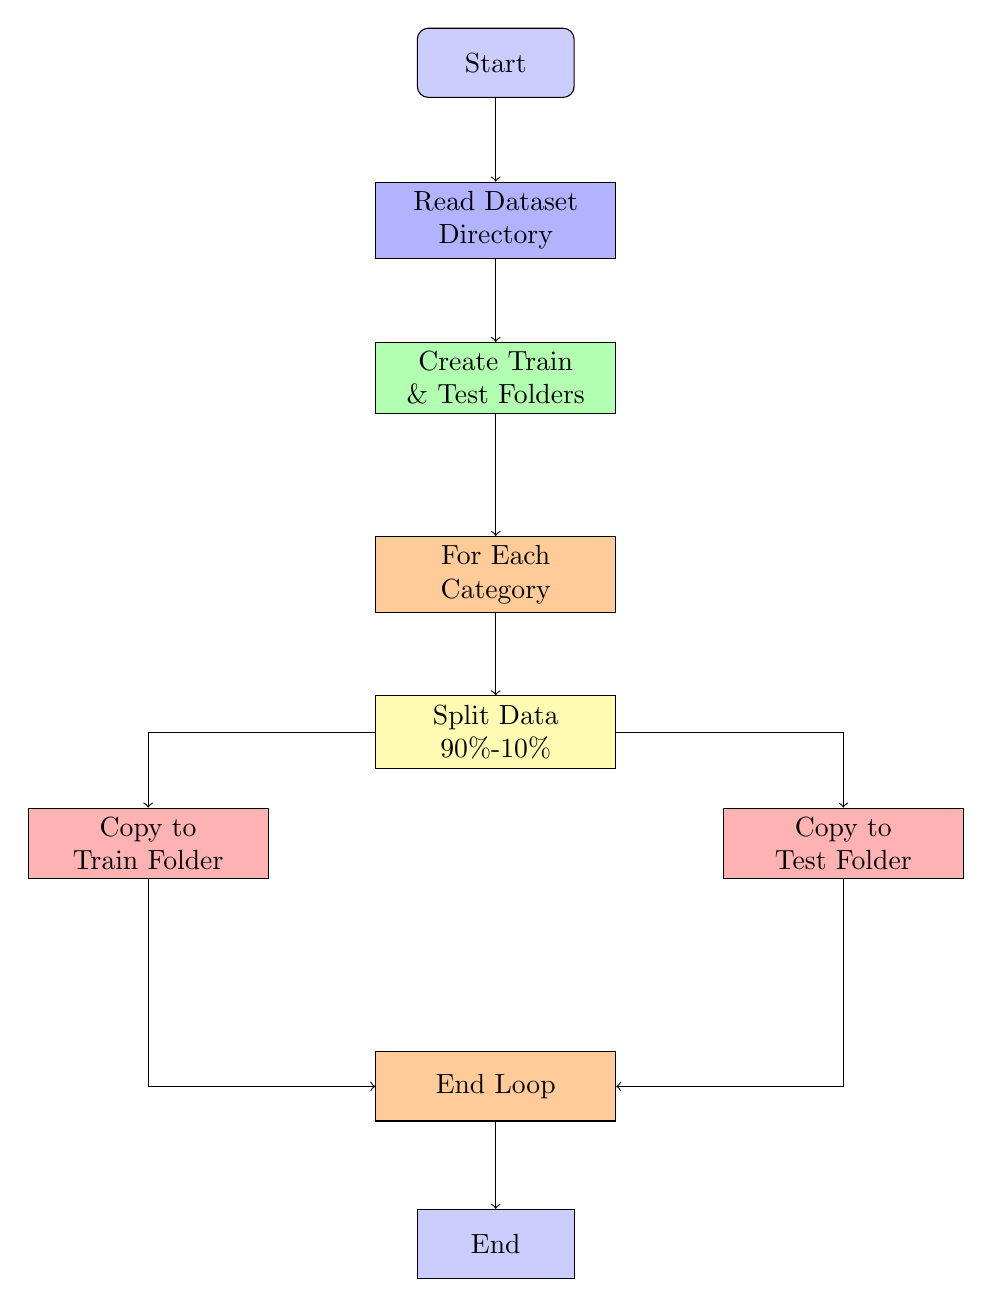
\begin{tikzpicture}[node distance=2cm, auto]
% Nodes
\node (start) [rectangle, draw, rounded corners, fill=blue!20, text width=5em, text centered, minimum height=2.5em] {Start};
\node (readdir) [rectangle, draw, below of=start, fill=blue!30, text width=8em, text centered, minimum height=2.5em] {Read Dataset Directory};
\node (createfolders) [rectangle, draw, below of=readdir, fill=green!30, text width=8em, text centered, minimum height=2.5em] {Create Train \& Test Folders};
\node (loopstart) [rectangle, draw, below of=createfolders, fill=orange!40, text width=8em, text centered, minimum height=2.5em, yshift=-0.5cm] {For Each Category};
\node (splitdata) [rectangle, draw, below of=loopstart, fill=yellow!30, text width=8em, text centered, minimum height=2.5em] {Split Data 90\%-10\%};
\node (copytrain) [rectangle, draw, below left of=splitdata, xshift=-3cm, fill=red!30, text width=8em, text centered, minimum height=2.5em] {Copy to Train Folder};
\node (copytest) [rectangle, draw, below right of=splitdata, xshift=3cm, fill=red!30, text width=8em, text centered, minimum height=2.5em] {Copy to Test Folder};
\node (endloop) [rectangle, draw, below of=splitdata, fill=orange!40, text width=8em, text centered, minimum height=2.5em, yshift=-2.5cm] {End Loop};
\node (end) [rectangle, draw, below of=endloop, fill=blue!20, text width=5em, text centered, minimum height=2.5em] {End};

% Arrows
\draw[->] (start) -- (readdir);
\draw[->] (readdir) -- (createfolders);
\draw[->] (createfolders) -- (loopstart);
\draw[->] (loopstart) -- (splitdata);
\draw[->] (splitdata) -| (copytrain);
\draw[->] (splitdata) -| (copytest);
\draw[->] (copytrain) |- (endloop);
\draw[->] (copytest) |- (endloop);
\draw[->] (endloop) -- (end);
\end{tikzpicture}
\end{center}